\documentclass[officiallayout]{tktla}
%\documentclass[officiallayout,a4frame]{tktla}
\usepackage[utf8]{inputenc}
\usepackage{latexsym}
\usepackage{graphicx}
\usepackage[
  backend=biber,
  bibstyle=ieee,
  citestyle=numeric-comp,
    sortlocale=en_US,
    natbib=true,
    url=false, 
    doi=true,
    eprint=false
]{biblatex}
\usepackage{software-biblatex}
\usepackage{pdfpages}
\usepackage[hidelinks]{hyperref}

% For thesis papers section
\usepackage{geometry}
\def \dvWHITE{white}
\def \dvBLACK{black}
\def \dvBLUE{blue}
\def \dvGREEN{green}
\def \dvheight{231pt}
% Creates black box with the text given as first parameter in white
\newcommand\note[3] {\marginpar{\vspace{#2}\colorbox{#3}{\parbox[c][\dvheight][t]{34.8pt}{\vspace{0.3cm}\color{white}\centering\Huge{\textbf{#1}}}}}}

% Footnotes without numbering
\let\svthefootnote\thefootnote

\addbibresource{maklin2022.bib}

\title{Probabilistic methods for \\ high-resolution metagenomics}
\author{Tommi Mäklin}
\authorcontact{tommi@maklin.fi\par
  https://maklin.fi/}
\pubtime{June}{2022}
\reportno{0}
\isbnpaperback{000-00-0000-0}
\isbnpdf{000-00-0000-0}
\issn{1238-8645}
\issnonline{2814-4031}
\printhouse{Unigrafia}
\pubpages{7} % --- remember to update this! 
% For monographs, the number of the last page of the list of references
% For article-based theses, the number of the last page of the list of
% references of the preamble part + the total number of the pages of
% the original articles and interleaf pages.
\supervisorlist{Antti Honkela, University of Helsinki, Finland \\ \hspace{8pt} Jukka Corander, University of Oslo, Norway}
\preexaminera{Exam Iner, University of Examinations, Exaministan}
\preexaminerb{Read Er, University of Examinations, Exaministan}
\opponent{Oppo Nent, University of Endless Argumentation, The Argumentlands}
\custos{Sea Land, University of Sealand, Sealand}
\generalterms{Algorithms, Experimentation}
\additionalkeywords{genomic epidemiology, plate sweeps, probabilistic modeling, pathogen surveillance, taxonomic profiling, taxonomic binning, metagenomics}
% Computing Reviews 1998 style
%\crcshort{A.0, C.0.0}
%\crclong{
%\item[A.0] Example Category
%\item[C.0.0] Another Example
%}
% Computing Reviews 2012 style
\crclong{
\item Mathematics of computing $\rightarrow$ Probability and statistics $\rightarrow$ Statistical computing
\item Computing applications $\rightarrow$ Biosciences
}

\permissionnotice{
  Doctoral dissertation, to be presented for public examination with 
  the permission of the Faculty of Science of the University of
  Helsinki in \ldots{} on \ldots{} at XX o'clock. Fill in the examination
  venue, date and time into the previous sentence.
}

\newtheorem{theorem}{Theorem}[chapter]
\newenvironment{proof}{\noindent\textbf{Proof.} }{$\Box$}

\begin{document}

\frontmatter

\maketitle

\begin{abstract}
  rewrite \citet{maklin_high-resolution_2021} a \citep{maklin_bacterial_2021}

\end{abstract}

\begin{acknowledgements}
  Olvi (III) \\ \& Koff IVA
   \begin{flushright}
  Rv  rip, June 2022\\
  Tommi Mäklin
  \end{flushright}
\end{acknowledgements}

\tableofcontents

\mainmatter

\chapter{Introduction}

In the past decades research focusing on bacterial pathogens has
largely been driven by analysis of the contents of bacterial genomes
obtained by whole-genome sequencing. Although the price of sequencing
itself has decreased tremendously during this timeframe, most analyses
still rely on using sequence data from pure bacterial cultures created
by isolating a bacterium from an initial mixed culture. Since these
cultures are created by cultivating environmental samples, they
typically contain several distinct bacteria \textemdash and other
microorganisms \textemdash that a thorough analysis would aim to
isolate in a pure culture. In practice, the number of isolations that
can be performed is limited and preparing large numbers of samples for
DNA sequencing rapidly becomes a significant economical barrier even
in well-resourced public health laboratories.

The typical use for sequencing data in public health settings is
genomic epidemiology, where researchers are interested analysing the
genomes of the pathogens to trace their transmission and spread. For
example, comparing mutations in the genomes of a pathogen isolated
from several patients during an epidemic may aid in inferring the
transmission chain by elucidating the short-term evolutionary
history. Similarly the long-term history can be inferred by looking
for larger structural changes, horizontal gene transfer, and
accumulated mutations in genomes assembled from the sequence data. If
the sequencing is performed routinely and the data is made publicly
available, the reporting from several laboratories may be combined to
create an extremely valuable resource for both researchers and
policymakers. However, the vast majority of genomic epidemiological
analyses require high coverage and high quality sequence data to
achieve meaningful resolution, which has translated to dominance of
the expensive pure-colony isolation approach in data generation.

Recently, shotgun metagenomics, where DNA is extracted and sequenced
directly from the original environmental sample, has emerged as a
potential cost-effective alternative to pure whole-genome
sequencing. Although this approach conveniently gets around both the
economic barrier and potential biases introduced by the cultivation
steps, direct sequencing often requires significantly higher
sequencing depths. Sequencing at depths typical to isolate analyses
often results in excess amounts of host DNA and fails to provide
sufficient resolution for the more elusive members of the microbiome
that are present only at low abundances. Due to these factors, shotgun
metagenomics may be difficult to apply in situations where researchers
are only interested in some subset of bacteria but wish to perform
analyses that require high sequencing depth.

When choosing between shotgun metagenomics and isolate sequencing, a
middle-ground can be found in creating the initial mixed culture but
skipping the isolation steps and instead sweeping and sequencing the
mixed culture. Since culture media are available for most clinically
relevant bacteria, this approach allows enrichment of the species of
interest while simultaneously filtering out host DNA, effectively
avoiding the pitfalls in both isolate and shotgun metagenomics by
limiting the diversity of the sample. Accordingly, this approach is
sometimes called limited-diversity metagenomics
\citep{cocker_drivers_2022} but will be referred to as plate sweep
metagenomics in this thesis.

Although both plate sweep metagenomics and shotgun metagenomics
have technically been possible for many years, the development of
computational methods has largely focused on analysing data from pure
cultures. Although some advances have been made in developing
computational tools capable of identifying the taxonomic composition
of a set of reads (taxonomic profiling) or assigning the individual
sequencing reads to their taxonomic origins (taxonomic binning), the
accuracy of these tools is significantly hindered in the presence of
within-species variation. In practice such variation is ubiquitous in
both clinical and envinronmental samples, rendering many of the tools
difficult to use when within-species level information is required.

In this thesis I present research that enables both taxonomic
profiling and binning from either metagenomic or plate sweep
sequencing data using computational methods. While the methods were
initially developed for plate sweeps metagenomics work, I also
demonstrate that they can reliably be applied to whole metagenome
sequencing data as well. Using either of the two approaches to
generate metagenomic sequencing data enables performing completely new
types of analyses which are also briefly covered.

The first two articles included in this thesis contain descriptions of
the aforementioned two methods. The first of these methods, called
mSWEEP, provides a probabilistic model for taxonomic profiling of
bacteria at within-species lineage level based on pseudoalignments
against a set of reference sequences. The second method, mGEMS,
leverages the information from mSWEEP to construct an assignment rule
for taxonomic binning of sequencing reads to bins that correspond to
the lineages. Both methods rely on the fundamentally important insight
that each sequencing read can - and should - pseudoalign and be
assigned to several lineages within the species at once. By combining
the two methods, sequencing data from samples containing several
lineages of the same species can be computationally demixed and used
to obtain results that are nearly indistinguishable from the results
of using isolate data.

While the methods from the first two articles are designed with direct
analysis of sequencing data from mixed cultures in mind, the third
article shows that both methods are applicable even when the initial
plating step is skipped and the sequencing data is derived directly
from an environmental sample. Thus, in the third article I have
analysed such samples from babies born in the UK collected during
their neonatal period and discovered several results showing strong
competition between bacterial species and strains during the initial
colonization of the gut microbiome. More importantly, from a methods
perspective, this analysis shows that mSWEEP and mGEMS provide
(so-far) completely unprecedented levels of resolution in analysis of
metagenomic sequencing data.

Together the three articles in this thesis represent foundational
methodological steps in both opening up high-resolution exploration of
bacterial diversity as well as making such analyses more accessible to
resource-constrained laboratories.

\section{Three approaches to sequencing bacterial DNA}

%- Something about sequeuncing reads and sequence assembly? 16S sequencing?

Preparing bacterial DNA for sequeuncing is typically done after a
culture step, where a sample is streaked across a culture plate or
immersed in liquid and then inoculated for some amount of time to
allow the bacteria to multiply and grow on the culture
plate. Alternatively, in metagenomics sequencing the culture step is
skipped and DNA is extracted directly from the sample along with the
DNA from any other organisms that may be present. When it comes to the
end-result, the sequencing reads, both approaches have their
advantages and disadvantages, which are covered in more detail in this
section.

Metagenomics sequencing, where all DNA in a sample is extracted
(Figure \ref{fig:microbiome-sampling-methods}a), has emerged as a tool
to analyse the full breadth of the microbiome. Metagenomics
conveniently avoids the biases introduced by approaches that include a
culture step and has consequently revealed an enormous diversity of
bacterial species that are not able to grow or compete on commonly
used culture media. However, exploring this diversity comes at a price
since the produced sequencing reads are split across the numerous
bacteria present, resulting in a prohibitively high sequencing depth
requirement for analysis of the less abundant taxa. This has rendered
the metagenomic approach difficult to apply in for example clinical
research, where the interesting bacteria (pathogens) are often only a
small part of the microbiome but the typical analyses require large
numbers of reads to produce accurate results.

Incorporating a culture step on a medium that selects for the bacteria
interest provides means to avoid wasting sequencing efforts on
uninteresting taxa. This approach allows for generating large numbers
of sequencing reads from the bacteria that grow to dominate the
culture, which in turn enables detailed analyses such as SNP calling
or identifying antimicrobial resistance genes. When the sequencing is
performed on the plate created from the sample, including all
bacterial species and strains that grow there, the approach is called
plate sweep metagenomics (Figure
\ref{fig:microbiome-sampling-methods}b). Although this approach has
not been previously widely used in the literature due to difficulties
in separating very closely related bacteria, it is a major application
area for the methods presented in this thesis due to the inherent
advantage of focusing sequencing resources on only the relevant
bacteria.

\noindent\let\thefootnote\relax\footnote{Figure source: Adapted from \cite{praveera_fenugreek-sprouts} and \cite{niaid_escherichia-coli}. Released under the \href{https://creativecommons.org/licenses/by-sa/4.0}{CC BY-SA 4.0 license}.}
\addtocounter{footnote}{-1}\let\thefootnote\svthefootnote
\begin{figure}[!ht]
  \label{fig:microbiome-sampling-methods}
    \centering
    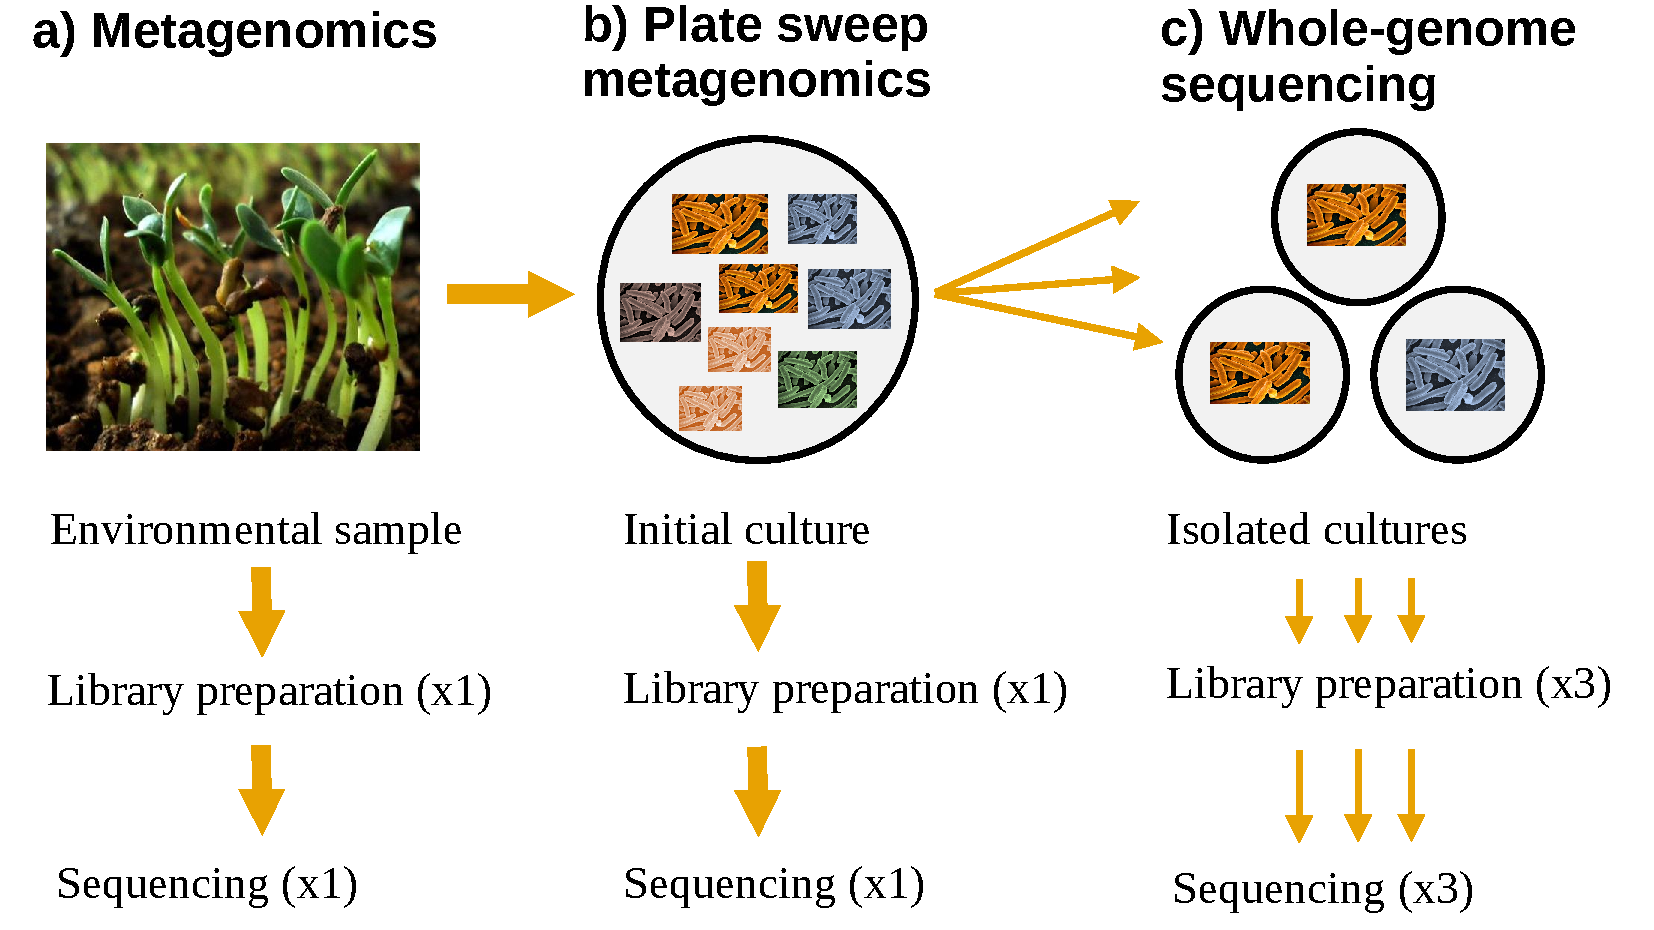
\includegraphics[width=\textwidth,keepaspectratio]{img/sampling/microbiome_sampling_methods.pdf}
    \caption{Different approaches to sequencing bacterial DNA. Panel \textbf{a)} depicts the metagenomic approach, where sequence data is collected directly from the environmental sample. Panel \textbf{b)} depicts the plate sweep metagenomic approach, where the environmental sample is plated on a selective medium and DNA is sequenced from the whole plate. Panel \textbf{c)} depicts the whole-genome sequencing approach, where a subset of visible colonies on the selective medium are picked, cultured again on their own plates, and then sequenced. The orange arrows depict steps that require laboratory work.}
\end{figure}

The third approach leverages a second culture step, where visible
colonies are picked from the initial culture and transferred to their
own culture plates. After letting the new plates inoculate, the
resulting culture will (presumably) contain only clones of the
bacteria that formed the colony that was picked. Since this approach
gets rid of all of the variation in both the sample and the initial
culture, resulting in massive numbers of sequencing reads from the
same genome, it is accordingly called whole-genome sequencing (Figure
\ref{fig:microbiome-sampling-methods}c). While this approach allows
accurate recovery of the genome of a single bacterial strain, the
number of colony picks that can be performed is often limited and some
sort of heuristic is required to select which colonies to pick.

In epidemiological analyses, the whole-genome sequencing approach has
so-far dominated the field due to its ability to produce highly
accurate data. However, transitioning sequencing efforts to either
metagenomics or plate sweep metagenomics has obvious benefits in both
upscaling the amount of samples that can be processed and in providing
better representation for both species and strain-level diversity in
the samples. Unfortunately the accuracy from existing tools has not
been as good as required but with recent developments in sequence
assembly and/or taxonomic binning \& profiling from metagenome-derived
sequencing data, the new frontier may finally be opening for
exploration.

\section{Analysing metagenomic sequence data}

\textbf{- Need a picture of the different approaches.}

Sequencing data from a metagenomic source presents several challenges
to bioinformaticians. Firstly, the increased diversity of species
requires much larger computational resources to analyse. Secondly, the
possible pressence of strain-level variation vastly complicates
analyses that rely on separating the reads to distinct taxonomic units
since the differences between strains of a bacteria can be minimal to
the level of being confused with sequencing error. Subsequently, most
of the methods development has focused on operating at the
species-level with the assumption that only one strain from each
species is present at the same time. In this section I will briefly
cover the previous approaches and introduce the principal differences
between them and mSWEEP and mGEMS.

Metagenome assemblers are one of the more used tools for analysing
metagenomic sequencing data. These assemblers aim to produce
assemblies directly from the sequencing reads, similarly to sequence
assembly in isolate sequencing but taking into account the different
taxons possibly present. Often, the assemblers work under the
assumption that the taxons in the reads are distinct enough that their
assembly graphs do not overlap. While this approach works fine when
the data contains taxons that are separated by long evolutionary
distances, it can fail in the presence of closely related strains of
the same species or even species of the same genus. Nevertheless,
metagenome assemblers have found a great deal of use in settings where
the data is assumed to contain many organisms that are, presumably,
unculturable or have not been encountered before.

Taxonomic profilers and taxonomic binners approach the metagenomics
problem from a slightly more detailed point of view. Taxonomic
profilers attempt to assign (relative) abundances to some sets of
reference data, or reference taxons, found in the reads, and taxonomic
binners attempt to create read bins that correspond to some reference
taxon. These two approaches often go hand-in-hand in that the
taxonomic profiles can be extracted by counting the reads in each bin
but some approaches still exist that attempt only the profiling
task.

Yet another category of metagenomics data analysis can be found in
approaches that do not attempt the previously mentioned tasks but
rather compare different samples to each other. These approaches
typically aim to infer similarity and, through that, transmission
events or shared strains between some samples. While these can be
extremely accurate especially in transmission analysis, these
approaches often cannot distinguish between different strains in the
sample and do not have the capability to perform analyses that require
access to the genomes of the individual strains. However, they can
provide information that would otherwise require analysing a large
number of genomes (in the case of perfect information i. e. a perfect
taxonomic binner) and have found much use in that regard.

Both profiling and binning methods can further be divided into
those that leverage reference data and those that attempt
reference-free estimation. While reference-free estimation can yield
data from previously unknow species or strains, reference-based
approaches typically obtain higher resolution. Leveraging reference
data is one of the central aspects of the work in this thesis to
perform both taxonomic profiling (mSWEEP) and taxonomic binning
(mGEMS), and the benefits of a reference-based approach will be
explored in more detail later on.

These metagenomics approaches have found widespread aplications in
analysing sequencing data from highly complex environments - such as
soil samples. Especially the reference-free approaches have proved
highly useful in cases where the contents of a sample bear little
similarity to previously sequenced samples. However, these scenarios
are becoming increasingly scarce with more widespread availability of
sequence data and new culture methods developed for species previously
thought unculturable. Especialy in clinical settings, where the
bacterial diversity is rather well known and has been studied for many
years, it is uncommon to come across an entirely new (pathogenic)
species. In these cases, adding information in the form of reference
sequences typically results in much higher ceiling for the possible
resolution.

In the class of metagenomics analyses, the approach presented in this
thesis falls broadly in reference-baesd taxonomic profiler and
taxonomic binner category. However, our approach differs from previous
research in that rather than trying to assign relative abundances to a
set of reference sequences, we attempt to assign abundances to a
reference \textit{lineage} - i. e. some group of reference sequences
that is somehow related to each other. This approach has the benefit
of covering the possible variation in a reference lineage, which
typically present problems for reference-based metagenomics
tools. Additionally, our tool works with bespoke sets of reference
sequences, which means that it can be applied to explore the diversity
of a specific species in great detail while excluding the
uninteresting species. While this discards some data that might be
useful, the approach greatly simplifies the modelling task, allowing
for a much higher accuracy in the exploration of within-species
variation.

\section{Genomic epidemiology as a tool for pathogen surveillance}

\textbf{Figure about genomic epidemiology analyses}

The other significant aspect of this thesis has to do with tracing the
spread of pathogens using sequence data, called genomic
epidemiology. In recent years, the use of genome-informed analyses has
greatly expanded the capability of researchers to track and trace
pathogens and identify genetic elements relevant for e. g. antibiotics
resistance and pathogenesis. This analysis has typically been
performed using isolate sequencing data, which provides great detail
into a single bacterial genome but has some downsides covered in the
previous sections. One important goal of the thesis work has been to
provide tools that extend the analysis capabilities to metagenomic
data from either plate sweeps or whole-genome shotgun sequencing.

Combining the genomic sequences of pathogens with data about the time,
location, and other clinically relevant features provides clinical
practitioners, policy makers, and researchers with a much wider
perspective into transmission and evolutionary analysis than using
either of the information alone. This has enabled several significant
advantages in e.g. analysis of the transmission of plasmids and
targeting vaccine design, as well as in providing novel insights into
several causative agents of disease that could not be identified
without including genome information. With the price of sequencing
constantly decreasing, genomics-driven analysis has high potential to
further revolutionize the way we think about disease.

Incorporating metagenomics data into genomic epidemiological analyses
presents the next obvious frontier. Since the microbiome is in
practice nearly universally composed of several interacting
micro-organisms, there is a high possibility that excluding some parts
may miss otherwise relevant information. For example, in a recent
study (Gerry's), the pathogen \textit{S. pneumonimae} was found to
often co-colonize patients with a dominant strain and a nondominant
strain. In the developed world, vaccine development has targeted the
dominant strain but entirely ignored the nondominant strain, which has
not been identified with previous methods. The nondominant strain
does, however, have the capability to cause the same disease and is,
in fact, the leading cause in the developing world. The results from
this study highlight that by focusing only on the non-metagenomic
contents of the microbiome, potentially significant information is
missed.

Another aspect in favour of using a more metagenomics-oriented
approach arises from simple practicality: sequencing several taxons at
once is simply more cost-effective than performing many isolations, as
covered in the previous sections. Using a metagenomics-oriented
approach makes the analyses much more widely available in the form of
significant cost reductions. This means that analyses which would not
be possible to perform in locations lacking funding and resources
might find a way through the use of metagenomic sequencing. Currently
especially data from lower-middle income countries is scarce due to
the limited sequencing capability which metagenomics has the potential
address. Furthermore, performing metagenomics sequencing alongside the
traditional sequencing types has the potential to preserve data from
the samples for future analyses, should methods capable for more
detailed exploration become available.

In conclusion, the already relatively recent field of genomic
epidemiology can be seen as underogoing a transform into becoming
widespread public practice. With the development of methods - such as
the ones presented in this thesis - capable of lowering the costs and
increasing the resolution, the field will likely produce significant
discoveries through the inclusion of metagenomics data.

\section{Contributions}

This thesis comprises three publications covering both mSWEEP and
mGEMS as well as a third article demonstrating their application to
whole-genome shotgun metagenomic sequencing data. The first two
publications are accompanied by software implementations. The third
article is more applied in nature, exploring in more detail the types
of analyses enabled by the first two papers.

\subsection*{Paper I \textemdash High-resolution sweep metagenomics using fast probabilistic inference}
By \underline{Tommi Mäklin}, Teemu Kallonen, Sophia David, Christine J
Boinett, Ben Pascoe, Guillaume Méric, David M Aanensen, Edward J Feil,
Stephen Baker, Julian Parkhill, Samuel K Sheppard, Jukka Corander, and
Antti Honkela. Published in \textit{Wellcome Open Research} (2021),
5:14, doi: 10.12688/wellcomeopenres.15639.2.

In the first paper, we presented and benchmarked the mSWEEP method for
taxonomic profiling of sequencing data containing multiple strains
from the same bacterial species. My contributions included development
and implementation of the method, designing the benchmarks and
comparisons with similar methods, running all analyses with mSWEEP,
writing the manuscript, and to reviewing and editing the article.

Software implementation of the ideas presented in Paper I is
available from GitHub at
\href{https://github.com/PROBIC/mSWEEP}{PROBIC/mSWEEP} (latest
version). The latest version at the time of writing is archived and
available in Zenodo \citep{maklin_mSWEEP}.

\subsection*{Paper II \textemdash Bacterial genomic epidemiology with mixed samples}
By \underline{Tommi Mäklin}, Teemu Kallonen, Jarno Alanko, Ørjan
Samuelsen, Kristin Hegstad, Veli Mäkinen, Jukka Corander, Eva Heinz,
and Antti Honkela. Published in \textit{Microbial Genomics} (2021)
7.11, doi: 10.1099/mgen.0.000691.

The second paper continued to build upon mSWEEP by developing an
algorithm for taxonomic binning at within-species variation level,
called mGEMS. I contributed to the development of both the mGEMS
binning algorithm and the full mGEMS pipeline, designing the synthetic
and the \textit{in vitro} benchmark experiments, running the analyses
and creating the visualisations, interpreting the results and writing
the article, and to reviewing and editing the article.

Software implementation of the ideas presented in Paper II is
available from GitHub at
\href{https://github.com/PROBIC/mGEMS}{PROBIC/mGEMS} (latest version).
The latest version at the time of writing is archived and available in
Zenodo \citep{maklin_mSWEEP}.

\subsection*{Paper III \textemdash Strong pathogen competition in neonatal gut colonization}
By \underline{Tommi Mäklin}, Harry Thorpe, Anna Pöntinen, Rebecca
Gladstone, Alan McNally, Ørjan Samuelsen, Pål Johnsen, Trevor Lawley,
Antti Honkela, and Jukka Corander. Awaiting peer-review; available
from \textit{bioRxiv} (2022), doi: XXX.XX/XXX.XXX.XXX.

The third paper provides an example of applying mSWEEP and mGEMS to
whole-genome shotgun metagenomics sequencing data and explores the
dynamics of pathogen competition and colonization in the gut
microbiome of babies in their first three weeks of life. My
contributions to this paper include running the mSWEEP/mGEMS pipeline
on all data used in the paper, updating the reference databases for
the investigated species, performing the analysis of the mSWEEP/mGEMS
results for the samples containing \textit{E. coli}, and aiding the
coauthors in analysing the other species. I additionally contributed
to creating the visualisations, interpreting the results, and
naturally to writing the article.

\section{Structure}

The rest of the thesis is structured into three chapters that describe
how the included papers contribute to the topics presented in the
introduction chapter. The first of the three chapters describes the
basic ideas behind the mSWEEP and mGEMS methods and provides
historical context for the parts of the methods that have their
origins within analysis of RNA sequencing data. The second chapter
describes the experimental results from the three papers in more
detail, focusing more on the applied part rather than the theoretical
foundations. The third chapter is more speculative in nature, covering
both the demonstrated epidemiological applications from the papers as
well as exploring potential future avenues for use of the developed
methods. The thesis concludes with a reprinting of the three included
articles.

\chapter{Mixture modeling of sequence data}

\section{Characteristics of sequence data from bacteria}

- write about Reference data vs Reference-free approach

- Write about individual sequence vs cluster based approach.
-- what is a strain? ie how to distinguish between them if we have no reference data

Something about bacterial pathogens are hard to classify taxonomically
and have weird genomes with weird plasmids and stuff.  Lineages are
much much nicer to work with

\section{Sequence alignment}

- Significance of alignment in the analyses (themisto vs traditional alignmnt? Could make a small example here)

- Significance of reference databases.

- Building bespoke databases vs. using refseq or something else.

\section{A probabilistic model for sequences from mixed sources}

- Diagram and equations of/from the mSWEEP model.

- Historical context from RNA sequencing.

- Add results from Gibbs sampler vs variational inference experiments.

This is a sample sentence that should look like normal text, and this
is another. This is a sample sentence that should look like normal
text, and this is another:
\[ S = \sum_{i=0}^{\infty} a^2 \]
This is a sample sentence that should look like normal text, and this
is another.\footnote{A sample footnote.}

\begin{theorem}
This is a sample sentence ($x=x+2$) that should look like normal text,
and this is another. This is a sample sentence that should look like
normal text, and this is another. This $x$ is a sample sentence $y$
that should look like normal text 32, and this is another.
\end{theorem}

\begin{proof}
This is a sample sentence that should look like normal text, and this
is another. This is a sample sentence that should look like normal
text, and this is another.
\end{proof}

\begin{theorem}
This is a sample sentence that should look like normal text,
and this is another:
\[ y = x+3 \]
\end{theorem}

\begin{proof}
This is a sample sentence.
\end{proof}

\section{From profiling to binning}

- How binning differs from profiling

- mGEMS algorithm and its interpretations

- Benefits of producing bins vs straight analysis of the sequence data

- Lineages vs taxons.

\section{The mSWEEP/mGEMS pipeline}

- Flowchart describing the analysis pipeline.

- Overview of the whole stuff and conclusion.

\chapter{High-resolution metagenomics}

More on mSWEEP/mGEMS \& how these tools enable new directions in research.

Refresher on plate sweeps and wgs metagenomics.

Something about metagenomics is nice in that we dont just sequence one
nice things but many nice things

Describe the benchmarking from the first two papers i e convince readers that the methods work nicely.

Could do some new kinds of benchmarks with the mGEMS paper synthetic data set.

cite \citet{tonkin-hill_pneumococcal_2022} for rigorous proof that
mSWEEP/mGEMS can recover cocolonization by several strains that is
overlooked by isolate sequeuncing.

\chapter{Metagenomic epidemiology}

Something about wgs and genomic epidemiology can do lots of cool stuff
to identify contaminated cucumbers or track covid.

Describe the experimental results from the first two papers.

Describe the experimental results from the third paper.

How do these show that what our methods are capable of and what they
could potentially be applied to in the future.

More speculative chapter.

\printbibliography[heading=bibintoc]

\chapter*{Included papers\markboth{Included papers}{}}
\addcontentsline{toc}{chapter}{Included papers}

\subsection*{Paper I \textemdash High-resolution sweep metagenomics using fast probabilistic inference}
By \underline{Tommi Mäklin}, Teemu Kallonen, Sophia David, Christine J
Boinett, Ben Pascoe, Guillaume Méric, David M Aanensen, Edward J Feil,
Stephen Baker, Julian Parkhill, Samuel K Sheppard, Jukka Corander, and
Antti Honkela. Published in \textit{Wellcome Open Research} (2021), 5:14
(https://doi.org/10.12688/wellcomeopenres.15639.2).

\subsection*{Paper II \textemdash Bacterial genomic epidemiology with mixed samples}
By \underline{Tommi Mäklin}, Teemu Kallonen, Jarno Alanko, Ørjan
Samuelsen, Kristin Hegstad, Veli Mäkinen, Jukka Corander, Eva Heinz,
and Antti Honkela. Published in \textit{Microbial Genomics} (2021)
7.11 (https://doi.org/10.1099/mgen.0.000691).

\subsection*{Paper III \textemdash Strong pathogen competition in neonatal gut colonization}
By \underline{Tommi Mäklin}, Harry Thorpe, Anna Pöntinen, Rebecca
Gladstone, Alan McNally, Ørjan Samuelsen, Pål Johnsen, Trevor Lawley,
Antti Honkela, and Jukka Corander. Awaiting peer-review; available
from \textit{bioRxiv} (2022) (https://doi.org/10.1099/mgen.0.000691).

%% \documentclass[officiallayout]{tktla}
%% \usepackage[utf8]{inputenc}
%% \usepackage{pdfpages}
%% % This package sets the margin width 
%% % (change "right" if you want them wider, but then change the 34.8pt in \note bigger too)
%% \usepackage[top=1.2in, bottom=1.5in, left=1in, right=1.6cm]{geometry}
%% \def \dvWHITE{white}
%% \def \dvBLACK{black}
%% \def \dvBLUE{blue}
%% \def \dvGREEN{green}
%% %%.72 = marker width§
%% %% 138,6: height 
%% % Use this if you have 5 articles
%% %\def \dvheight{138.6pt}
%% % Use this if you have 6 articles
%% \def \dvheight{115.5pt}
%% % Creates black box with the text given as first parameter in white
%% \newcommand\note[3] {\marginpar{\vspace{#2}\colorbox{#3}{\parbox[c][\dvheight][t]{34.8pt}{\vspace{0.3cm}\color{white}\centering\Huge{\textbf{#1}}}}}}

%% % This overlays a white box to make black box narrower, but it's not needed anymore with geometry package changing margin width
%% %\newcommand\notee[2]{\marginpar{\vspace{#1}\colorbox{#2}{               \parbox[c][\dvheight][t]{11.8pt}{              \color{white}\centering\Huge{\textbf{$\ $}}}}}}

%% \pagestyle{empty}
%% \begin{document}


\newgeometry{top=1.2in, bottom=1.5in, left=1in, right=1.6cm}

% ******************************************************************************
\chapter*{Paper I}\thispagestyle{plain}
\addcontentsline{toc}{section}{High-resolution sweep metagenomics using fast probabilistic inference}

\note{I}{-222pt}{black}
%\notee{-222pt}{\dvWHITE}

% Here it's not necessary to draw the following boxes to position right,
% and drawing them occasionally creates unwanted gray lines

%\note{II}{-100pt}{\dvWHITE}
%\notee{-126.5pt}{\dvWHITE}

%\note{III}{-5pt}{\dvWHITE}
%\notee{-126.5pt}{\dvWHITE}

%\note{IV}{-5pt}{\dvWHITE}
%\notee{-126.5pt}{\dvWHITE}

%\note{V}{-5pt}{\dvWHITE}
%\notee{-126.5pt}{\dvWHITE}

%\note{VI}{-5pt}{\dvWHITE}
%\notee{-126.5pt}{\dvWHITE}

\vspace{80pt}
% The names of the authors
\underline{Tommi Mäklin}, Teemu Kallonen, Sophia David, Christine J
Boinett, Ben Pascoe, Guillaume Méric, David M Aanensen, Edward J Feil,
Stephen Baker, Julian Parkhill, Samuel K Sheppard, Jukka Corander, and
Antti Honkela.

\vspace{10pt}
% Title of the 1st paper
\noindent\textbf{High-resolution sweep metagenomics using fast probabilistic inference}

\vspace{10pt}
% Bibliographical information of the paper, for example, of a conference paper
\noindent In
\emph{Wellcome Open Research},
\\vol. 5 issue 14, 2021.

\vspace{60pt}
% Copyright information, if the publisher is, for example, ACM
\noindent Copyright \textcopyright\ 2021 Mäklin T et al. This is an
open access article distributed under the terms of the Creative
Commons Attribution License, which permits unrestricted use,
distribution, and reproduction in any medium, provided the original
work is properly cited.

\cleardoublepage
% Including the original publication
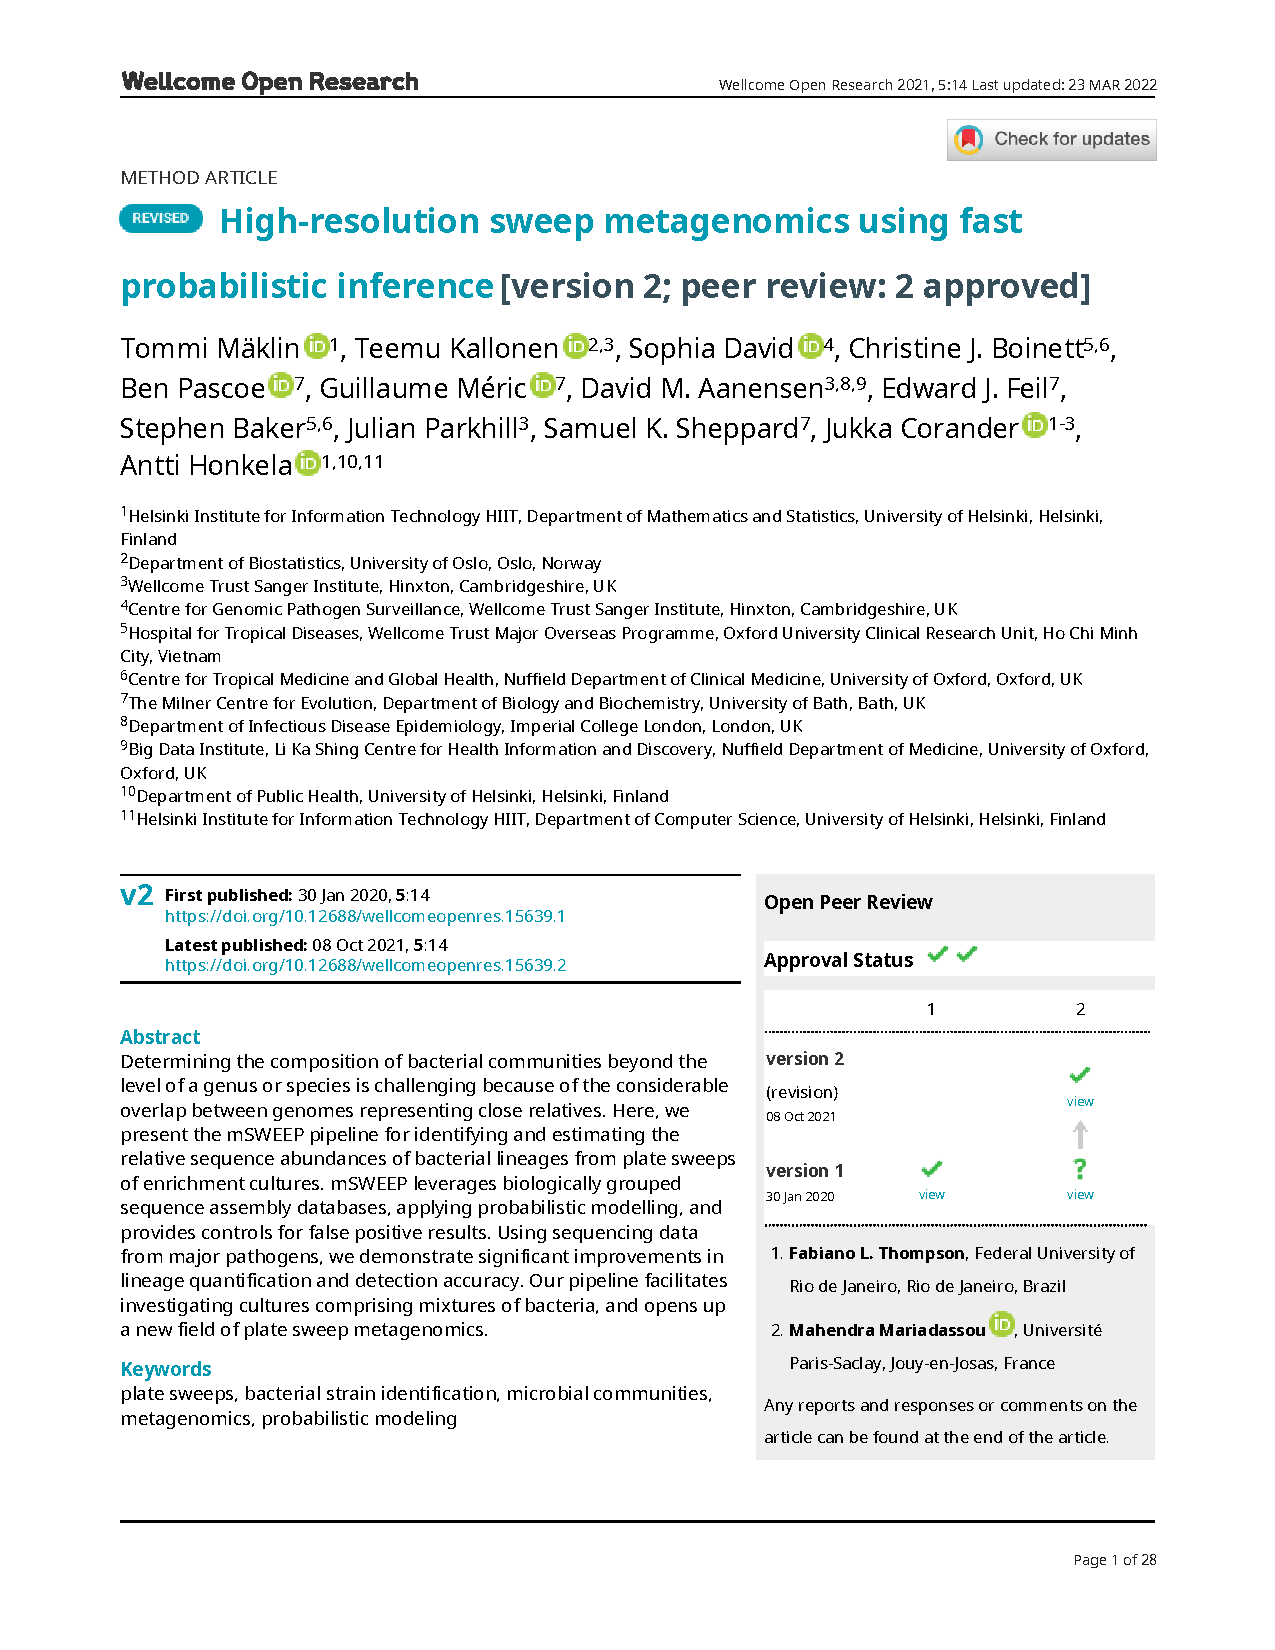
\includepdf[pages=-]{papers/maklin_high-resolution_2021.pdf}


% ******************************************************************************


\chapter*{Paper II}\thispagestyle{plain}
\addcontentsline{toc}{section}{Bacterial genomic epidemiology with mixed samples}

\note{I}{-222pt}{\dvWHITE}
%\notee{-222pt}{\dvWHITE}

\note{II}{-5pt}{black}
%\notee{-126.5pt}{\dvWHITE}

\note{III}{0pt}{\dvWHITE}
%\notee{-126.5pt}{\dvWHITE}

%% \note{IV}{-5pt}{\dvWHITE}
%% %\notee{-126.5pt}{\dvWHITE}

%% \note{V}{-5pt}{\dvWHITE}
%% %\notee{-126.5pt}{\dvWHITE}

%% \note{VI}{-5pt}{\dvWHITE}
%% %\notee{-126.5pt}{\dvWHITE}

\vspace{80pt}

% Here are the names of the authors
\underline{Tommi Mäklin}, Teemu Kallonen, Jarno Alanko, Ørjan
Samuelsen, Kristin Hegstad, Veli Mäkinen, Jukka Corander, Eva Heinz,
and Antti Honkela.

\vspace{10pt}
% Title of the 2nd paper
\noindent\textbf{Bacterial genomic epidemiology with mixed samples}

\vspace{10pt}
% Bibliographical information of the paper, for example, of a conference paper
\noindent In 
\emph{Microbial Genomics}, 
\\vol. 7 issue 11, 2021.

\vspace{60pt}
% Copyright information, for example, if the publisher is Springer
\noindent Copyright \textcopyright\ The Authors. This is an
open-access article distributed under the terms of the Creative
Commons Attribution License. This article was made open access via a
Publish and Read agreement between the Microbiology Society and the
corresponding author’s institution.

\cleardoublepage
% Including the original publication
\includepdf[pages=-]{papers/maklin_bacterial_2021.pdf}

% ******************************************************************************


\chapter*{Paper III}\thispagestyle{plain}
\addcontentsline{toc}{section}{Strong pathogen competition in neonatal gut colonization}

\note{I}{-222pt}{\dvWHITE}
%\notee{-222pt}{\dvWHITE}

\note{II}{-5pt}{\dvWHITE}
%\notee{-126.5pt}{\dvWHITE}

\note{III}{0pt}{black}
%\notee{-126.5pt}{\dvWHITE}

%% \note{IV}{-5pt}{\dvWHITE}
%% %\notee{-126.5pt}{\dvWHITE}

%% \note{V}{-5pt}{\dvWHITE}
%% %\notee{-126.5pt}{\dvWHITE}

%% \note{VI}{-5pt}{\dvWHITE}
%% %\notee{-126.5pt}{\dvWHITE}

\vspace{80pt}
% Here are the names of the authors
\underline{Tommi Mäklin}, Harry Thorpe, Anna Pöntinen, Rebecca Gladstone, Alan McNally, Ørjan
Samuelsen, Pål Johnsen, Trevor Lawley, Antti Honkela, and Jukka Corander.

\vspace{10pt}
% Title of the 3rd paper
\noindent\textbf{Strong pathogen competition in neonatal gut colonization}

\vspace{10pt}
% Bibliographical information of the paper, for example, a submitted paper
\noindent Submitted, preprint available from \emph{bioRxiv}.

\vspace{60pt}
%Copyright information, when the authors have the copyright of the paper
\noindent
The copyright holder for this preprint is the author/funder, who has
granted bioRxiv a license to display the preprint in perpetuity. It is
made available under a CC-BY 4.0 International license.

\cleardoublepage
% Including the original publication
%\includepdf[pages=-]{Publication_name_3.pdf}



% ******************************************************************************


%% \chapter*{Paper IV}\thispagestyle{empty}
%% \note{I}{-222pt}{\dvWHITE}
%% %\notee{-222pt}{\dvWHITE}

%% \note{II}{-100pt}{\dvWHITE}
%% %\notee{-126.5pt}{\dvWHITE}

%% \note{III}{-5pt}{\dvWHITE}
%% %\notee{-126.5pt}{\dvWHITE}

%% \note{IV}{-5pt}{black}
%% %\notee{-126.5pt}{\dvWHITE}

%% \note{V}{-5pt}{\dvWHITE}
%% %\notee{-126.5pt}{\dvWHITE}

%% \note{VI}{-5pt}{\dvWHITE}
%% %\notee{-126.5pt}{\dvWHITE}

%% \vspace{80pt}
%% % Here are the names of the authors
%% John Doe, Jane Doe, and John Smith

%% \vspace{10pt}
%% % Title of the 4th paper
%% \noindent\textbf{This is the title of the 4th paper}

%% \vspace{10pt}
%% % Bibliographical information of the paper, for example, of a journal paper
%% \noindent
%% In \emph{Journal name}, \\Volume xx, 20ZZ, pages XX-YY.

%% \vspace{60pt}
%% % Copyright information, when the authors have the copyright
%% \noindent Copyright \textcopyright\ The Authors.

%% \cleardoublepage
%% % Including the original publication
%% \includepdf[pages=-]{Publication_name_4.pdf}

% ******************************************************************************

\restoregeometry

%\end{document}


\end{document}
